\label{sec:Vorueberlegung}

\textbf{Ontologien}

Die bereits im Grundlagenkapitel erw{\"a}hnten Ontologien sind aufgrund ihrer
Komplexit{\"a}t und umfangreichen Einbindungszeit nicht Bestandteil des im
Verlaufe dieser Arbeit entwickelten Protokolls. Jedoch ist eine Einbindung
selbiger im weiteren Entwicklungsverlauf des Protokolls unabdingbar. Diese sind
jedoch kein Bestandteil dieser Arbeit.
Das zuk{\"u}nftige Ziel ist es mit Hilfe der Ontologien eine automatisierte
Priorisierung von Daten vorzunehmen. Somit kann ein auf dem Mars
befindliches System (z.B. ein Rover) selbstst{\"a}ndig entscheiden, welche
Informationen eine hohe Priorit{\"a}t zugewiesen bekommen.

\textbf{Time To Live}

Die \gls{TTL} bezeichnet die Lebensdauer eines Datenpakets und ist
dabei von unterschiedlichen Aspekten abh{\"a}ngig. So kann ein Paket einerseits nach
Ablauf eines Zeitraums oder nach einer bestimmten Anzahl
von Hops verworfen werden. Das Ablaufen durch den Hop\footnote{Ein Hop
bezeichnet eine Station einer Route auf dem Weg zum Ziel (Knoten)}-Zähler
ist dabei in einem Szenario der interplanetaren Kommunikation derzeit eher
unrealistisch, da zumeist eine Punkt-zu-Punkt Verbindung anvisiert wird (kein
intensives Routing {\"u}ber eine Vielzahl an Stationen). Somit w{\"a}re unter
Ber{\"u}cksichtigung einer interplanetaren Kommunikation eine \gls{TTL} Realisierung
per Zeitstempel sinnvoller, da hier{\"u}ber, unter Ber{\"u}cksichtigung des
{\"U}bertragungskontextes, unrealistische {\"U}bertragungszeiten einfach erkannt
werden k{\"o}nnen.
Aufgrund der beschr{\"a}nkten Ressourcen unter interplanetaren
Kommunikationsumgebungen ist die Frage nach der Vorhaltedauer von
entscheidender Bedeutung. Damit wird die Speicherung der
Daten auf Seiten des extraterrestrischen Senders bezeichnet. 
Eine m{\"o}gliche Entscheidungsgrundlage daf{\"u}r, wann Daten aus einer
\gls{FIFO} verworfen werden sollen, w{\"a}re die Wichtigkeit selbiger. So
k{\"o}nnen Daten geringer Relevanz direkt nach dem Senden gel{\"o}scht werden.
Wohingegen Daten hoher Relevanz erst nach Empfangsquittierung bzw. Ablauf des
\gls{TTL} Timers verworfen werden.

\textbf{Protocol Stack} \label{sec:Konzept_Protocolstack}

Die von der jeweiligen Anwendung an den \gls{CROP} Stack {\"u}bergebenen Daten
werden zun{\"a}chst in kleinere Datenbl{\"o}cke gesplittet. Diese Datenbl{\"o}cke
werden der Relevanz nach evaluiert und anschlie{\ss}end priorisiert.
Im Anschlu{\ss} daran werden die priorisierten Datenbl{\"o}cke der jeweiligen
Wertigkeit in einer \gls{FIFO} gespeichert. Danach werden im
\gls{glos:Packetizer} die Datenbl{\"o}cke h{\"o}chster Priorit{\"a}t zu einer
Nachricht zusammengefasst, die danach an den \gls{UDP} Stack {\"u}bergeben werden
kann. Dieser grundlegende Ablauf ist in Abbildung \ref{fig:CRODT} schematisch
dargestellt.

\begin{figure}[H]
\centering
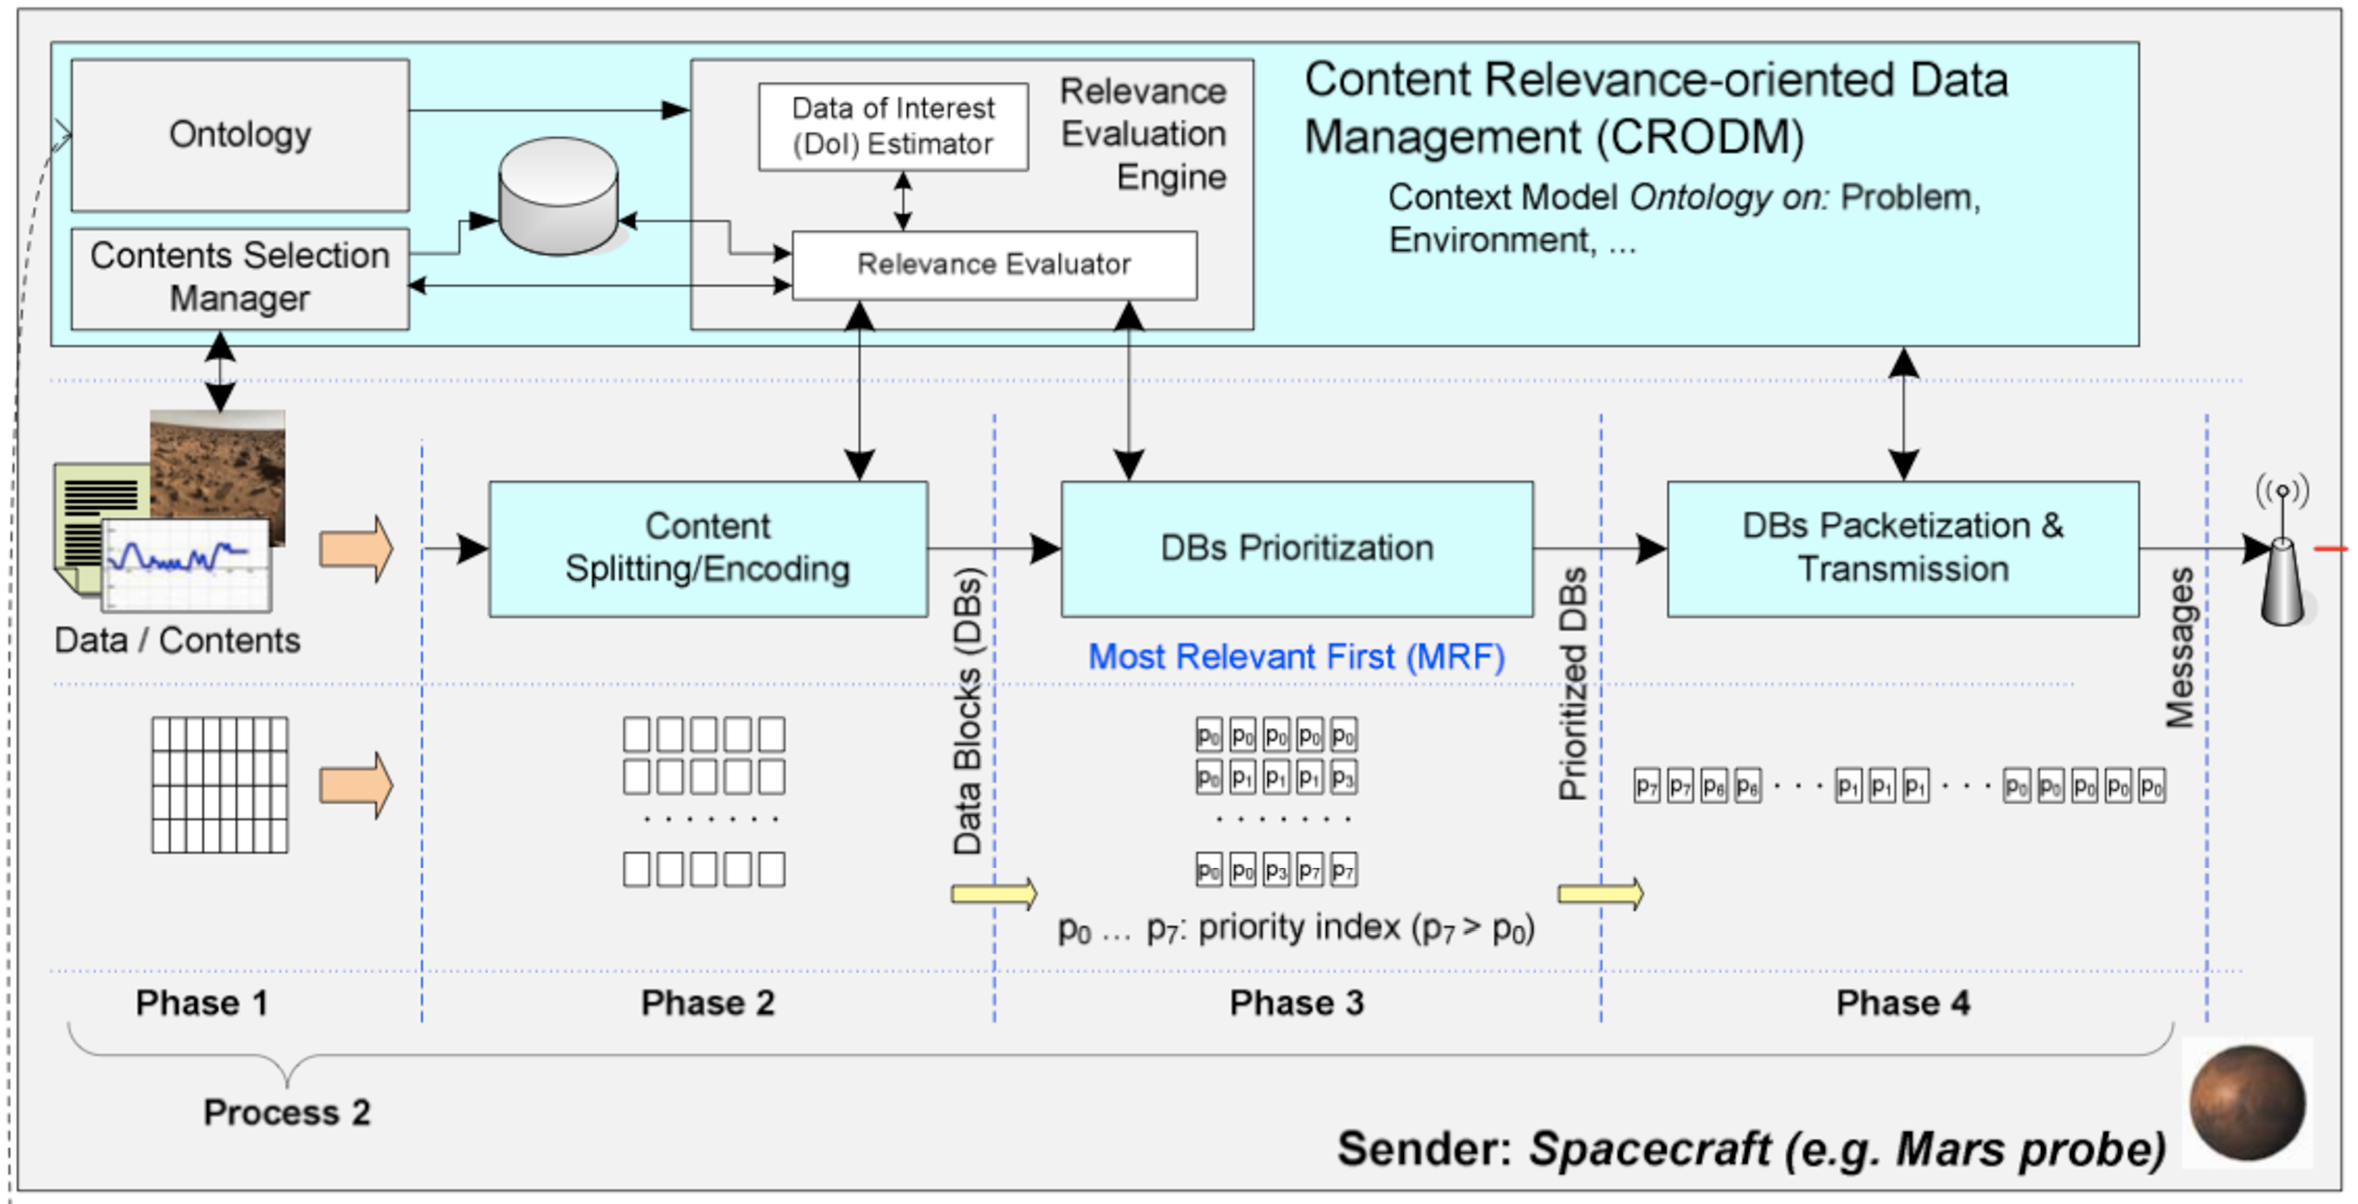
\includegraphics[scale=.3]{CRODT.pdf}
\caption{Das CRODT Framework (Ref. \cite{Daher})}
\label{fig:CRODT}
\end{figure}

In Abbildung \ref{fig:OSI_Stack} wird die Schachtelung der Daten
innerhalb des OSI-Stacks aufgezeigt. Dabei wird das Weiterreichen der Daten an
die jeweils n{\"a}chste Schicht des Stacks verdeutlicht. In jedem dieser Schritte wird dem neuen
Datenpaket der Header der aktuellen Schicht angeh{\"a}ngt und somit das
weitergereichte Datenpaket um notwendige {\"U}bersetzungsinformationen f{\"u}r
den Empf{\"a}nger erweitert. Auf der Empf{\"a}ngerseite erfolgt eine Invertierung dieses
Vorganges. 

\begin{figure}[H]
\centering
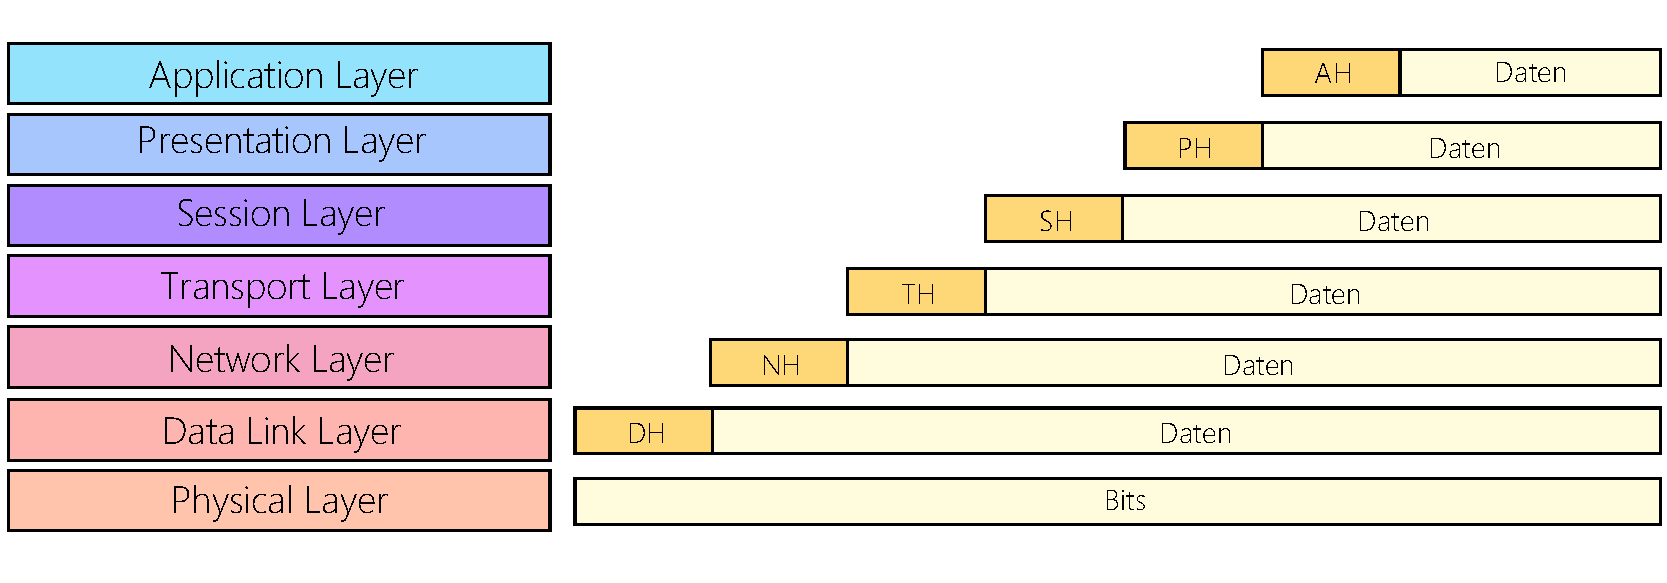
\includegraphics[scale=.5]{OSI_Stack.pdf}
\caption{Der OSI Stack}
\label{fig:OSI_Stack}
\end{figure}
 
Die Abbildung \ref{fig:CROP_Stack} zeigt die Handhabung im CROP-Stack
unter Nutzung des \gls{UDP}-Protokolls f{\"u}r die finale Daten{\"u}bertragung. Der
Application, Presentation und Session Layer des OSI-Modells
wird hierbei vereinfacht als Anwendungsschicht zusammengefasst.
Der Transport Layer des OSI-Modells entspricht der Transportschicht des
vereinfachten Modells. Die Internetschicht repr{\"a}sentiert den Network
Layer.
Der Data Link Layer und der Physical Layer des OSI-Modells wird zur
Netzzugangsschicht zusammengefasst. Dem OSI-Modell entsprechend wird eine
equivalente Darstellung der Paketerweiterung um den jeweiligen Header
hinzugef{\"u}gt. Der Protokollablauf sieht dabei nach Aufteilung der Daten in
Bl{\"o}cke und Zuweisung einer Priorit{\"a}t, eine Zusammenfassung zu einer
Nachricht mit ausschließlich höher priorisierten Daten vor. Dieses Datenpaket
wird nun an den \gls{UDP}-Stack weitergegeben. Diese werden
anschlie{\ss}end um den \gls{IP}-Header erweitert und dann entsprechend
der {\"U}bertragungsschnittstelle und deren Protokoll versandt.

\begin{figure}[H]
\centering
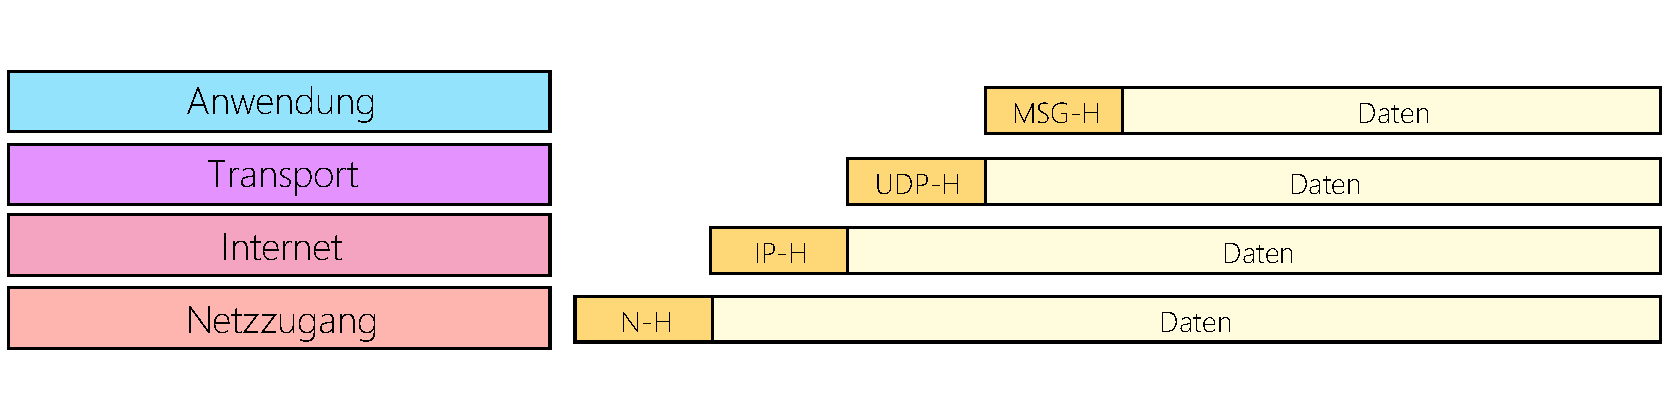
\includegraphics[scale=.5]{CROP_Stack.pdf}
\caption{Der CROP Stack}
\label{fig:CROP_Stack}
\end{figure}

\textbf{Error Correction Code}

Zur Fehlererkennung bzw. -korrektur wird ein CRC-Code verwendet. Dieser wird
innerhalb des Protokolls abhängig der Paketgr{\"o}{\ss}e auf CRC 16 Bit oder
CRC 32 Bit eingestellt. Die Pr{\"u}fsumme wird durch einen mathematischen
Algorithmus ermittelt und dann mit dem Paket {\"u}bertragen. Wenn der
Empf{\"a}nger die R{\"u}ckrechnung unter Einbeziehnung der Pr{\"u}fsumme
vornimmt, kann anhand des Ergebnisses ermittelt werden, ob das Paket
verf{\"a}lscht wurde. Die Berechnung einer Checksumme funktioniert dabei wie
folgt:

Das zu {\"u}bertragende Datenframe sei exemplarisch gegeben als: 11 0101 1011.
Desweiteren wird ein CRC-Generatorpolynom ben{\"o}tigt, welches im Beispiel als
$G(x) = x^4 + x + 1$ gegeben sei. Die daraus resultierende Schreibweise in Generatorbits lautet: 10011
($1*x^4+0*x^3+0*x^2+1*x^1+1*x^0$).
Anschließend wird eine erweiterte Darstellung des zu {\"u}bertragenden Frames
erzeugt, woraus der folgende Ausdruck hervorgeht: 11 0101 1011 0000
(Frame-0-Bits; Erweiterung des Datenframes um die Ordnung des Generatorpolynoms
in Nullen). Danach erfolgt eine Division des erweiterten Frames durch das
Generatorpolynom, welche nachfolgend dargestellt ist.

\makeatletter
\def\cline#1{\noalign{\vskip-2ex}\@cline#1\@nil}
\makeatother

\begin{figure}[H]
\jot-0.6mm
\begin{alignat*}{14}
1&1&0&1&0&1&1&0&1&1&0&0&0&0& : 10011=1100001010 \\
1&0&0&1&1\\ \cline{1-5}
&1&0&0&1&1& \\ 
&1&0&0&1&1& \\ \cline{2-6}
&&0&0&0&0&1& \\ 
&&1&0&0&1&1& \\ \cline{3-7}
&&&0&0&0&1&0& \\                                                 
&&&1&0&0&1&1& \\ \cline{4-8}
&&&&0&0&1&0&1& \\                                               
&&&&1&0&0&1&1& \\ \cline{5-9}
&&&&&0&1&0&1&1& \\                                           
&&&&&1&0&0&1&1&  \\ \cline{6-10}                                                                                  
&&&&&&1&0&1&1&0& \\                                           
&&&&&&1&0&0&1&1& \\   \cline{7-11}                                                                                      
&&&&&&&0&1&0&1&0& \\                                         
&&&&&&&1&0&0&1&1& \\ \cline{8-12}                                                                                     
&&&&&&&&1&0&1&0&0& \\                                       
&&&&&&&&1&0&0&1&1& \\ \cline{9-13}                                                                               
&&&&&&&&&0&1&1&1&0& \\                                     
&&&&&&&&&1&0&0&1&1& \\ \cline{10-14}    
&&&&&&&&&&1&1&1&0& 
\end{alignat*}
\caption{Modulo-2-Division} 
\end{figure}

Der Rest $1110$ dieser Modulo-$2$-Division wird an das
urspr{\"u}nglich zu {\"u}bertragende Frame $11 0101 1011$ angeh{\"a}ngt. Somit
ergibt sich das Frame inklusive Pr{\"u}fsumme: $11 0101 1011 1110$. Der
Empf{\"a}nger kann damit {\"u}berpr{\"u}fen, ob das Frame korrekt {\"u}bertragen
wurde. Dazu wird dieses durch das Generatorpolynom (Generatorbits) geteilt.
Das Ergebnis muss dabei null sein. Das im Beispiel genutzte Polynom kann mit der
Ordnung $4$ ($2^4=16$) auf Daten von $16$ Bit Länge angewendet werden. Das
Polynom $x16+x12+x5+1$ wird hingegen beispielsweise beim CRC-CCITT $16$ Bit-Verfahren
genutzt und kann auf Datenframes bis zu einer Gr{\"o}{\ss}e von $2^{16}=65536$
Bit angewendet werden (Ref. \cite{web2}).

